\chapter{Example Workflows}
\index{Workflows}

\section{Creating a Hydrogeological Subsurface Mesh}

\subsection{Input Data}

To set up a model with \ogs, certain information needs to be present in the programme. As \ogs performs simulations on finite element meshes, such a mesh needs to be either created with \ogs or with other software, after which it needs to be imported into the programme. \ogs supports a large number of typical geo-scientific data formats (see figure \ref{fig:interfaces} for an overview).

For importing data created with other software (such as shape files, borehole data, non-OGS meshes, etc), go to \cmd{File \ra Import files...} and select the appropriate file type. A file-open-dialogue will pop up and after selecting the respective file it is imported into \ogs.

If the imported data will be needed later on in \ogs (e.g. For setting boundary conditions) or if it has been somehow modified using the \emph{Data Explorer}, the data set needs to be saved in \ogs format. Select the \emph{Data View} tab where the data set is listed (i.e. Geometry, Meshes, Stations or Modelling) and click the little disk-sympbol on top of the tab. Geometric data will be saved in a gml-file, meshes in vtu-files, station-data in stn-files and modelling data (i.e. Boundary conditions) in cnd-files. Repeat this process for every data set you would like to convert and save in an \ogs format.

\subsection{Creating a 2D Finite Element Mesh}
%
\begin{figure}[htb]
\begin{center}
\subfloat[Boundary only]{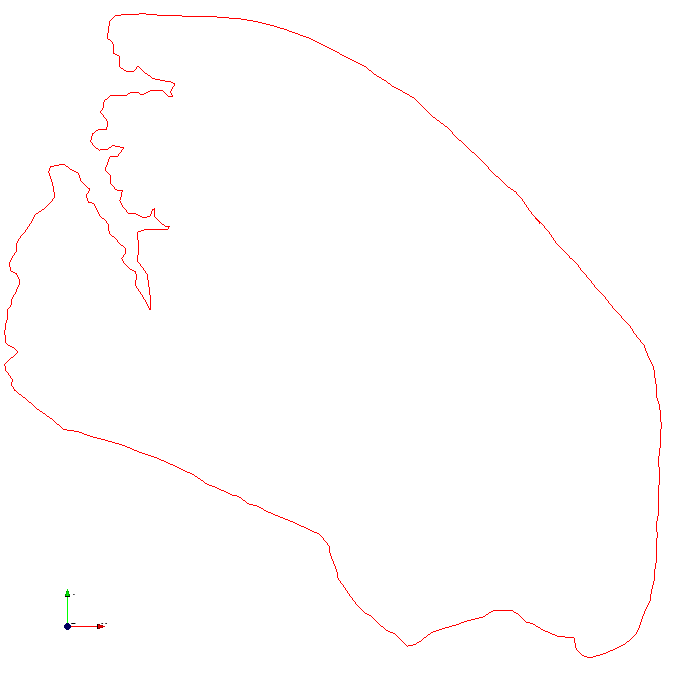
\includegraphics[width=0.3\linewidth]{ammer_geo1}}\enspace
\subfloat[With streams added]{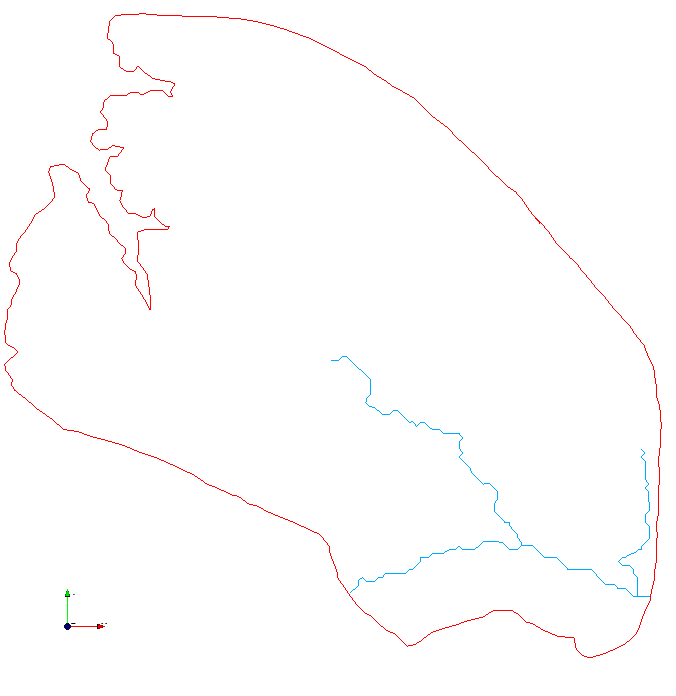
\includegraphics[width=0.3\linewidth]{ammer_geo2}}\enspace
\subfloat[With boreholes added]{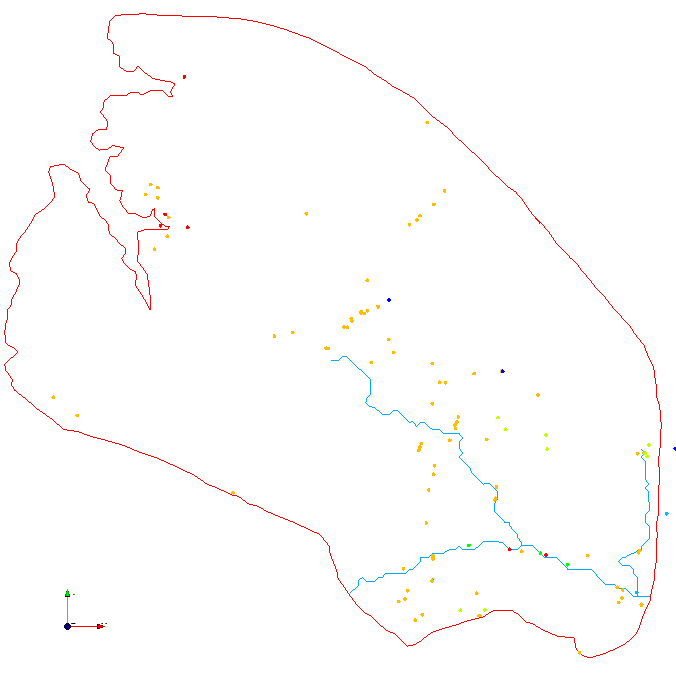
\includegraphics[width=0.3\linewidth]{ammer_geo3}}\\
\subfloat[Mesh from boundary]{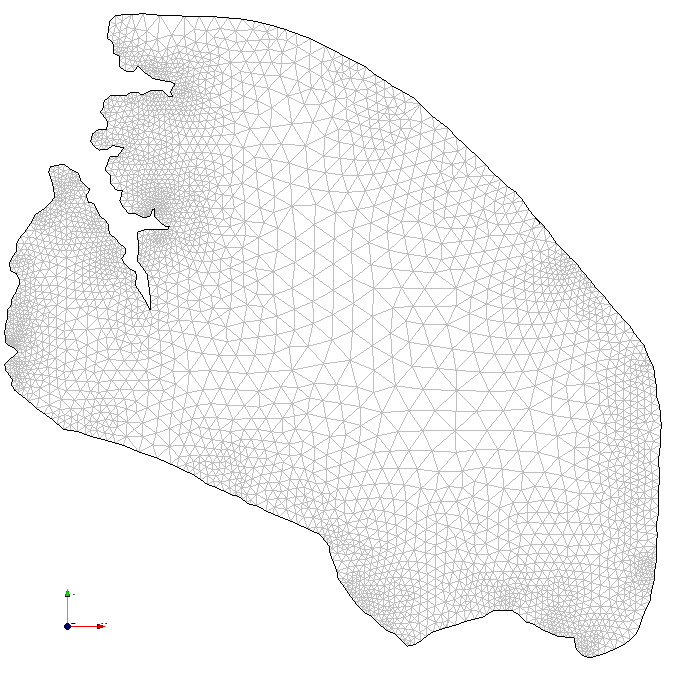
\includegraphics[width=0.3\linewidth]{ammer_mesh1}}\enspace
\subfloat[Including streams]{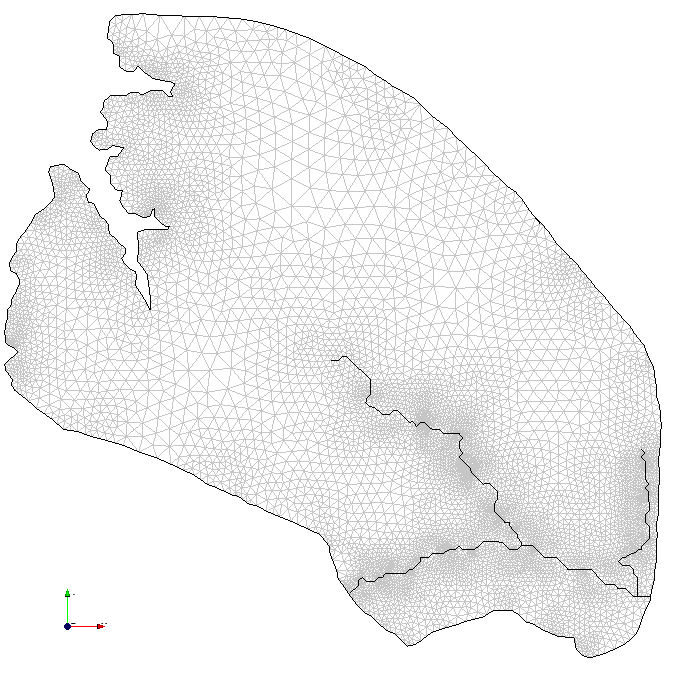
\includegraphics[width=0.3\linewidth]{ammer_mesh2}\label{fig:ammer-mesh2}}\enspace
\subfloat[Including streams and boreholes]{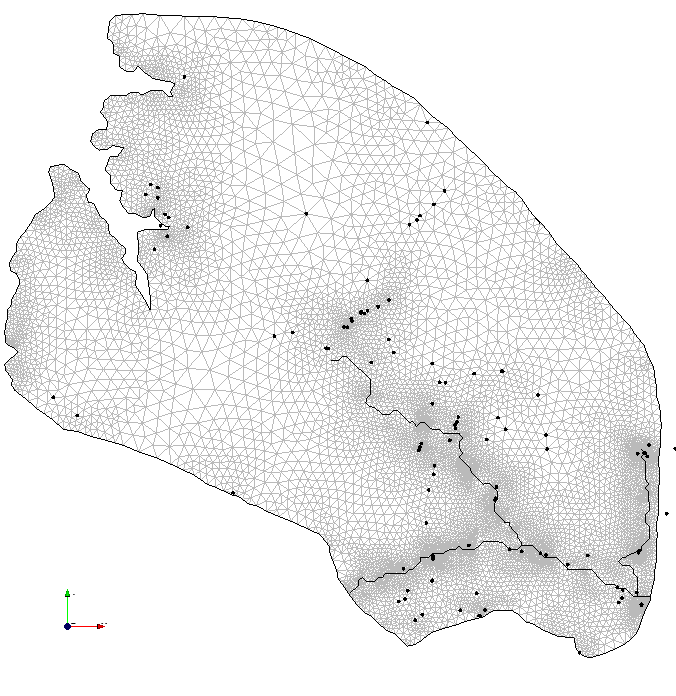
\includegraphics[width=0.3\linewidth]{ammer_mesh3}\label{fig:ammer-mesh3}}\\
\subfloat[Mesh from boundary]{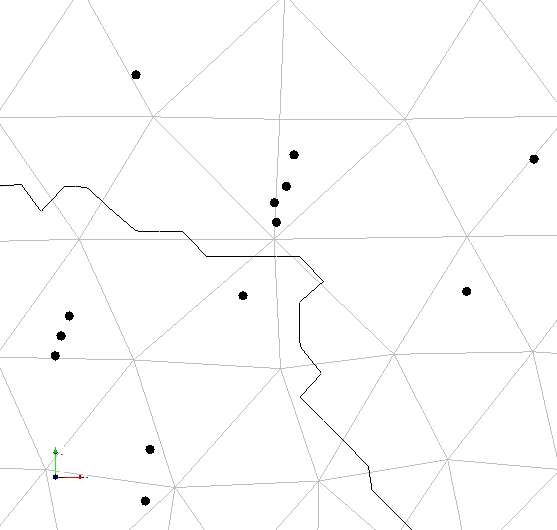
\includegraphics[width=0.3\linewidth]{ammer_meshgeo1}}\enspace
\subfloat[Including streams]{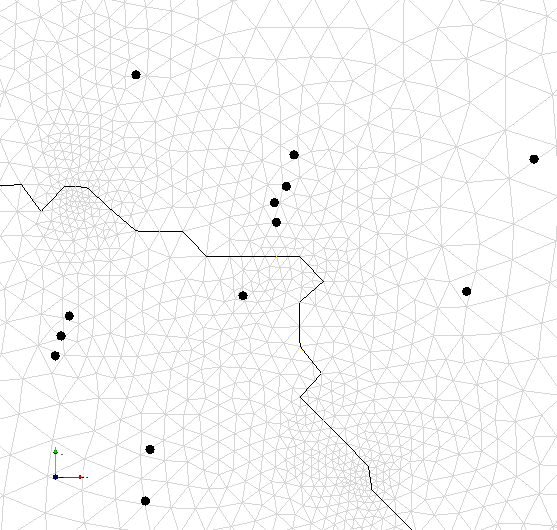
\includegraphics[width=0.3\linewidth]{ammer_meshgeo2}}\enspace
\subfloat[Including streams and boreholes]{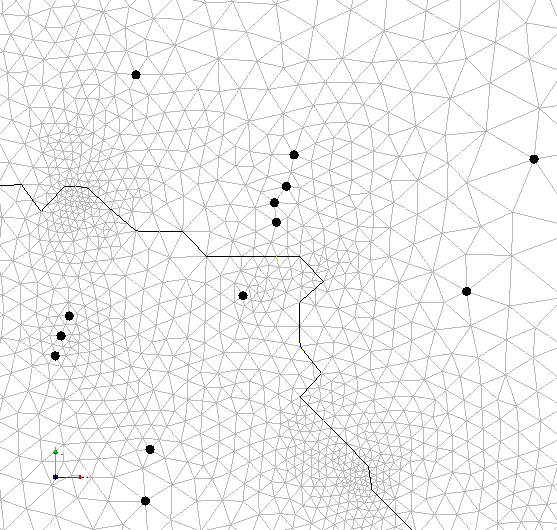
\includegraphics[width=0.3\linewidth]{ammer_meshgeo3}}\\
\end{center}
\caption{Effect of adding more information to the meshing process. The upper row shows geometric input data, with one data set added in each column. The resulting meshes are depicted in the second row. The meshes in figures \ref{fig:ammer-mesh2} and \ref{fig:ammer-mesh2} have a similar refinement but in one mesh boreholes located directly on mesh nodes and in the other mesh they are not. The bottom row gives a close-up of this effect to visualise how geometric information matches mesh nodes and edges if it has been integrated into the meshing process.\label{fig:workflow:2Dmesh}}
\end{figure}

The minimum requirements for creating a 2D mesh is a closed polyline representing the outer boundary of the model region as well as a digital elevation model to derive the elevation at any point within the region.

A 2D surface mesh from these two data sets is now created by
\begin{enumerate}
\item Create a triangulation for the area bounded by the polyline \label{step1}
\item Map the resulting 2D mesh using the DEM to create a model for the actual surface \label{step2}
\end{enumerate}

When creating the triangulation in step \ref{step1}, it is also possible to integrate additional data into the mesh that is relevant for the model. See figure \ref{fig:workflow:2Dmesh} for the effect of integrating additional information during the meshing process. Generating meshes from geometry is described in detail in section \ref{meshcreation}.

The resulting mesh will be a 2D triangle mesh with elevation $z=0$ for all mesh nodes. To create a surface mesh representing the actual surface of the domain, the elevation of mesh nodes is mapped based on a DEM of the region. For that, right-click on the 2D-mesh in the Mesh Data View and select \cmd{Edit mesh...}. When asked for the number of mesh layers, select $0$ as the resulting mesh does not actually contain a subsurface layer but just the surface itself. The dialogue will then ask for the location of the DEM used for mapping and upon clicking
\cmd{OK}. Details on that topic are given in section \ref{meshondemmapping}.


\subsection{Creating and Mapping Subsurface Layers}

To create a 3D subsurface mesh, a 2D mesh of the domain is required. This surface need not be mapped before creating a 3D mesh.

Again, right-click on the 2D mesh that needs to be extruded to 3D and select \cmd{Edit mesh...}. Select the number of subsurface layers to be added to the mesh and press \cmd{Next}.

There are two options for adding new layers to a 2D meshes:
\begin{enumerate}
\item Layers may have a constant thickness (i.e. all layers may have different thickness but thickness within a layer is constant)
\item Layer thickness may be based on elevation maps of subsurface layer boundaries in raster format (i.e. DEMs of layer boundaries, usually interpolated from borehole data)
\end{enumerate}

Depending on which option has been chosen, either the thickness of each layer has to be specified or, alternatively, the path to a DEM raster for each layer boundary. In addition to layer boundaries, it is also possible to specify a DEM (i.e. Surface elevation) which will be used for cutting all information from interpolated layers that is located above actual surface level. Details on adding layers of fixed thickness can be found in section \ref{fixedsizelayers}, information for adding layers based on subsurface DEMs can be found in section \ref{meshondemmapping}.

Note, that subsurface layers can only be added to 2D meshes, i.e. once layers are added, the dimension of the mesh changes to 3D and no more additional layers can be added.


%\section{Assigning FEM Conditions}
%
%conditions on geometrical objects
%
%setting conditions directly on meshes nodes

\section{Visualisation of Results}

If the output of simulation results is given in VTK-format, it is possible to load the files containing the results into the \emph{Data Explorer} via \cmd{Import files...\ra VTK}. Currently, time-steps have to be loaded seperately. Once loaded, all \ogs-visualisation options are available for manipulation of the result. This includes general visualisation options (detailed in section \ref{genvisoptions}) as well as visualisation filters (see section \ref{filters}).
The programme will automatically determine if the data loaded is a mesh or geometric data and will handle visualisation and filter options accordingly.
